\documentclass{beamer} 
\usetheme{default} 
\usecolortheme{albatross}
\setbeamercovered{transparent}
%\useoutertheme{umbcfootline}  


\usepackage[spanish]{babel}
%\usepackage[latin1]{inputenc}
\usepackage[utf8x]{inputenc}
\usepackage{hyperref}
\usepackage{color}



\usepackage{multicol}


\title{POO II}

\author{Manuel J. Molino Milla \and Luis Molina Garzón}

\date{\today} %

\institute{IES Virgen del Carmen \and Departamento de Informática}




%\beamerdefaultoverlayspecification{<+->}

\begin{document}


\begin{frame}
  \titlepage
\end{frame}

\begin{frame}
    \frametitle{Logo}
\begin{figure}

\includegraphics[scale=1]{imagenes/logo.jpeg} 
\caption{Logo Java}
\end{figure}
\end{frame}

\begin{frame}
  \frametitle{Contenido}
  \tableofcontents[pausesections]
\end{frame}



\section{Introduccion}

\begin{frame}
\frametitle{Diferencia entre tipo primitivo y objeto}
\begin{itemize}[<+->]
\item Cada variable representa una posición de memoria que almacena un valor.
\item Cuando se declara una variable le decimos al compilador que \emph{tipo} se debe almacenar \alert{int numero;}
\item De esa manera se reserva el espacio de memoria exacta para ese tipo, \emph{ejemplo 4 bytes para tipos int}
\item Para el caso de objeto, se define el tipo como \emph{TipoObjeto Objeto}
\item Puede ser 4 byte o 8 byte suele ser el tamaño dependiendo si la arquitectura es 32 o 64 bits.
\item Dicha referencia guarda la posición de memoria donde se localiza el objeto.
\item Todos los casos anteriores hablamos de \alert{la pila de memoria}
\item Mientrás que para objetos hablamos de \alert{el mónticulo} o \emph{memoria dinámica}
\end{itemize}
\end{frame}

\begin{frame}
\frametitle{Tipos primitivos y referencias}
\begin{figure}
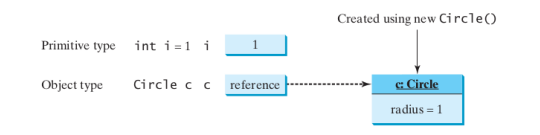
\includegraphics[scale=0.7]{imagenes/referencia1.png}
\end{figure}

\begin{multicols}{2}
\begin{figure}
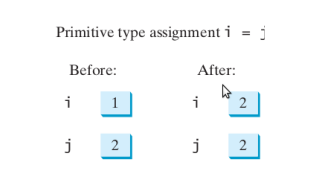
\includegraphics[scale=0.6]{imagenes/referencia2.png}
\end{figure}
\begin{figure}
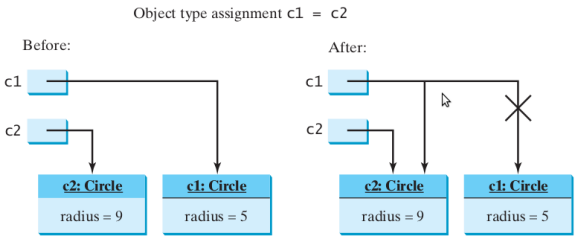
\includegraphics[scale=0.36]{imagenes/referencia3.png}
\end{figure}
\end{multicols}
\end{frame}

\section{Array de objetos}
\begin{frame}
\frametitle{Array de objetos}
\begin{itemize}[<+->]
\item Ejemplo: \emph \{Circle[ ] circleArray = new Circle[10];\}
\item Un array de objetos es un array de referencias.
\end{itemize} 
\begin{figure}
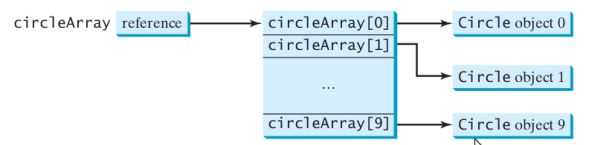
\includegraphics[scale=0.6]{imagenes/referencia4.png}
\end{figure} 
\end{frame}

\section{Encapsulacion}

\begin{frame}[fragile]
\frametitle{Encapsulamiento de datos} 
\begin{multicols}{2}
\begin{tiny}
\begin{verbatim}
public class Circulo {
/** Radio del círculo */
  private double radio = 1;
/** Número de objetos creados */
  private static int numberoDeObjetos = 0;
/** Constructor de un círculo de radio 1 */
  public Circulo() {
     numberDeObjetos++;
  }
/** Constructor de un círculo de radio dado */
  public Circulo(double nuevoRadio) {
     radio = nuevoRadio;
  }
/** Devueve el radio -access method-*/
  public double getRadio() {
     return radio;
  }
/** Set a nuevo radio radius -mutator method-*/
  public void setRadio(double nuevoRadio) {
    radio = (nuevoRadio >= 0) ? nuevoRadio : 0;
}
/** Devuelve numero de Objetos */
  public static int getNumeroDeObjetos() {
    return numeroDeObjetos;
}
/** Devuelve el area del círculo */
  public double getArea() {
    return radio * radio * Math.PI;
    }
}	
\end{verbatim}
\pause
\begin{itemize}[<+->]
\item Hay dos datos \emph{encapsulados}: radio y numeroDeObjetos.
\item Sólo accesible mediante métodos de acceso.
\item Métodos denominados generalmente \alert{getters}
\end{itemize}
\end{tiny}
\end{multicols}

\end{frame}


\section{Objetos como parametros}

\begin{frame}[fragile]
    \frametitle{Objetos como parámetros de método}

\begin{itemize}[<+-| alert@+>]
      \item Se pueden pasar objetos como argumentos de métodos.
      \item Realmente estamos pasando la referencia del objeto.
      \item Ejemplo:    
\end{itemize}
\pause
\begin{verbatim}
public class Test {
   public static void main(String[] args) {
     Circulo miCiculo = new Circulo(5.0);
     printCirculo(miCirculo);
   }

   public static void printCirculo(Circulo c) {
     System.out.println("El área del círculo de radio "
          + c.getRadio() + " es " + c.getArea());
   }
}
\end{verbatim}
\pause
\begin{itemize}[<+-| alert@+>]
	\item Los argumentos se pasan por \alert{valor}
	\item El valor pasado es la referencia.
	\end{itemize}
\end{frame}


\begin{frame}[fragile]
    \frametitle{Paso por valor o referencia}
  \begin{block}{VALOR}
El paso de parámetros por valor consiste en copiar el contenido de la variable que queremos pasar en otra dentro del ámbito local de la subrutina, consiste pues en copiar el contenido de la memoria del argumento que se quiere pasar a otra dirección de memoria, correspondiente al argumento dentro del ámbito de dicha subrutina. Se tendrán dos valores duplicados e independientes, con lo que la modificación de uno no afecta al otro.
  \end{block}
  \pause
  \begin{block}{REFERENCIA}
El paso de parámetros por referencia consiste en proporcionar a la subrutina a la que se le quiere pasar el argumento la dirección de memoria del dato. En este caso se tiene un único valor referenciado (o apuntado) desde dos puntos diferentes, el programa principal y la subrutina a la que se le pasa el argumento, por lo que cualquier acción sobre el parámetro se realiza sobre la misma posición de memoria.
  \end{block}
\end{frame}

\section{Variables y metodos estaticos}

\begin{frame}
    \frametitle{Variables y metodos estaticos}
    \begin{itemize}[<+-| alert@+>]

      \item En la clase objeto teniamos dos variables:
      \item \emph{private double radio = 1;}
      \item \emph{private static int numberoDeObjetos = 0;}
      \item A la primera se llama \emph{variable de instancia}
      \item  A la segunda se le llama \emph{variable de clase}
	 \item Las \emph{variables de instancia} son particulares para cada objeto, no de la clase,  ni para el resto de objetos de las clase.      
      \item Ejemplo el radio de un círculo es independiente de otro círculo.
      \item Si queremos que todos lo objetos comparten algún dato, usamos variables de clase también llamadas variables estáticas.
      \item Se usa un lugar común de la memoria para almacenar los valores de las variables estáticas
      \item Debido a su posición común, cualquier objeto puede acceder a dichos valores.
      \item Java soporta variables y  métodos estáticos que pueden ser llamados sin crear un objeto de la clase.
\end{itemize}
\end{frame}



\begin{frame}
    \frametitle{UML con miembros estaticos}
    Los miembros estaticos aparecen subrayados.
\begin{figure}
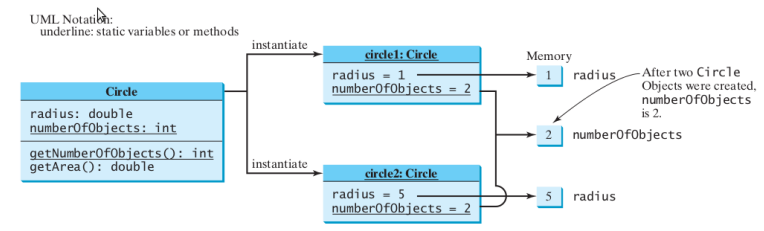
\includegraphics[scale=0.55]{imagenes/umlstatic.png}
\end{figure}
Para acceder a los miembros estáticos usariamos:\\
\alert{Circle.numberOfObjects} y \alert{Circle.getNumberOfObjects()
}
\end{frame}


\begin{frame}[fragile]
    \frametitle{Miembros estaticos}
\begin{itemize}[<+->]
\item Los miembros estáticos pueden accederse desde objetos y métodos estáticos.
\item Sin embargo los métodos estáticos no pueden acceder a miembros de instancia.
\item El siguiente código da error:
\end{itemize}  
\pause
\begin{scriptsize}
\begin{verbatim}
public class Foo {
   int i = 5; //variable de instancia
   static int k = 2; //variable de clase
   public static void main(String[] args) {
   		int j = i; // Mal porque i es una variable de instancia
        m1(); // Mal porque  m1() es un método de instancia 
   public void m1() {
     i = i + k + m2(i, k); //i, j son accesible
     //pues m1 es un método de instancia
   }
   public static int m2(int i, int j) {
     return (int)(Math.pow(i, j));
     //Mal pues i es una variable de instancia
   }
}
\end{verbatim}
\end{scriptsize}
\end{frame}

\begin{frame}[fragile]
    \frametitle{Miembros de clase o miembros de instancia}
   \framesubtitle{¿Cuando escoger un miembro estático o de instancia?}
   \pause
   Cuando dicho miembro no dependa del objeto debe ser de instancia
\begin{multicols}{2}
\begin{scriptsize}
\begin{verbatim}
public class Test {
  public int factorial(int n) {
     int resultado = 1;
     for (int i = 1; i <= n; i++)
        resultado *= i;
     return resultado;
  }
}
\end{verbatim}
\begin{verbatim}
public class Test {
  public static int factorial(int n){
     int resultado = 1;
     for (int i = 1; i <= n; i++)
        resultado *= i;
     return resultado;
  }
}
\end{verbatim}
\end{scriptsize}
\end{multicols}
\pause
\alert{Deberíamos escoger la segunda opción pues el  método factorial no depende de ningún objeto tipo Test.}
\end{frame}


\section{this}

\begin{frame}[fragile]
\frametitle{Referencia this}
\begin{itemize}[<+->]


\item \alert{this} tiene el sentido de ''este objeto'' o ''el objeto actual''
\item Produce una referencia al objeto actual.
\item Venimos usándolo en los getters y en los constructores.
\end{itemize}
\begin{tiny}
\begin{multicols}{3}
\begin{verbatim}
public class Numero{
  private int valor;
  public Numero(int valor){
    this.valor=valor;
  }
}
\end{verbatim}
\begin{verbatim}
public class Numero{
  private int valor;
  public Numero(int v){
    this.valor=v;
  }
}
\end{verbatim}
\begin{verbatim}
public class Numero{
  private int valor;
  public Numero(int v){
    valor=v;
  }
}
\end{verbatim}
\end{multicols}
\end{tiny}
\begin{itemize}[<+->]
\item Cuando hacemos Numero n1 = new Numero(5);
\item En el constructor se hace this.valor=5;
\item \alert{this} hace referencia a \alert{n1}
\end{itemize}
\end{frame}


\begin{frame}[fragile]
\frametitle{Diferencia con métodos estáticos}
En los metodos estaticos usamos \alert{NombreClase}.\alert{MiembroEstático}
\begin{tiny}
\begin{verbatim}
public class Numero
{
  private int valor;
  private static int numeroObjetos = 0;
  public void setValor (int valor)
  {
    this.valor = valor;
    Numero.numeroObjetos++;
  }
  public int getValor ()
  {
    return this.valor;
  }
  public static int getNumeroObjetos ()
  {
    return Numero.numeroObjetos;
  }
  public static void main (String[]args)
  {
    Numero n1 = new Numero ();  //Creo el objeto
    Numero n2 = new Numero ();  //Creo el objeto
    n1.setValor (5);            //Le doy valor 5 al atributo valor
    n2.setValor (15);           //Le doy valor 15 al atributo valor
    System.out.println ("Valor del número: " + n1.getValor ());
    System.out.println ("Valor del número: " + n2.getValor ());
    System.out.println ("Numero de objetos: " + Numero.getNumeroObjetos ());
  }
}
\end{verbatim}
\end{tiny}
\end{frame}




\begin{frame}[fragile]
    \frametitle{Otros usos de this}
    \emph{this} nos da la posibilidad de invocar a un constructor dentro de la misma clase:
   \begin{verbatim}
public class Circulo {
   private double radios;
   public Circulo(double radio) {
     this.radio = radio;
   }
   public Circul0() {
     this(1.0);
   }
   public double getArea() {
     return this.radio * this.radio * Math.PI;
   }
\end{verbatim} 
\end{frame}


\section{Composicion}

\begin{frame}
    \frametitle{Composición}
\begin{multicols}{2}
\begin{footnotesize}
\begin{itemize}[<+->]
\item Un objeto puede contener a otros objetos.
\item La relación entre ambos se llama \alert{composición}.
\item Ejemplo:
\item Tenemos una clase \emph{Agenda}
\item Tenemos una clase \emph{contatos}
\item Una Agenda agrupa a varios Contactos
\end{itemize}
\end{footnotesize}
\begin{figure}
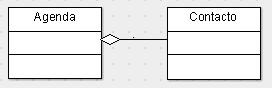
\includegraphics[scale=0.5]{imagenes/uml1.jpg}
\caption{UML de composición}
\end{figure}

\begin{figure}
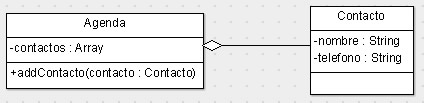
\includegraphics[scale=0.4]{imagenes/uml2.jpg}
\caption{Código de composición}
\end{figure}
\end{multicols}
\end{frame}


\section{Clases internas}

\begin{frame}[fragile]
\frametitle{Clases internas}
\begin{footnotesize}
\begin{itemize}[<+->]
\item Una clase interna es una clase que se define dentro de otra.
\item Permite agrupar clases relacionadas.
\item Se suelen considerar como miembros de la clase a la que pertenece.
\item Por lo que puede  añadir los modificadores \emph{public, package, protected o private.}
\end{itemize}
\end{footnotesize}
\pause
\begin{small}
\begin{multicols}{2}
\begin{verbatim}
class Externa {
    . . .
    class Interna {
        . . .
    }
}
\end{verbatim}
Se pude usar con:
\begin{verbatim}


class Externa {
    . . .
    class Interna {
        . . .
    }
    void metodo() {
      Interna i = new Interna();
        . . .
    }
}
\end{verbatim}
\end{multicols}
\end{small}
\pause
\begin{footnotesize}
\begin{itemize}
\item La compilación crea dos clases: Externa.class y Externa\$Interna.class
\item Desde fuera se puede acceder como \emph{Externa.Interna ei = (new Externa()).new Interna();}
\end{itemize}\end{footnotesize}
\end{frame}

\begin{frame}[fragile]
\frametitle{Clase internas}
\framesubtitle{Clases internas estáticas}
\begin{verbatim}
public class Externa {

  public static class Interna {

  }

}
\end{verbatim}
\pause
Para crear una instancia de la clase interna, lo tratamos como un miembro estáticos de una clase.\\
\pause
La instancia se crearía:
\pause
\emph{Externa.Interna instancia = new Externa.Interna();}\\
Podemos acceder a los atributos estáticos de la clase que lo envuelve.
\end{frame}

\begin{frame}[fragile]
\frametitle{Clase internas}
\framesubtitle{Clases internas locales}
\begin{small}
Son definidas dentro de un método o dentro de un bloque \{\dots\}

\begin{verbatim}
class Externa {

    public void metodo() {

        class Local {

        }

        Local local = new Local();
    }

}
\end{verbatim}
\end{small}
\pause
\begin{footnotesize}
\begin{itemize}[<+->]
\item Solo son accesible en el ámbito donde se definen: el método o bloque \{\dots\}
\item La clase local puede acceder a miembros (atributos o métodos) definidos en la clase externa.
\item También se pueden declarar como \emph{clases estáticas locales}.
\end{itemize}
\end{footnotesize}
\end{frame}

\begin{frame}[fragile]
\frametitle{Clase internas}
\framesubtitle{Clases internas anónimas}
%\begin{small}
Como su nombre indica, son clases sin nombre.
\begin{verbatim}
ActionListener click = new ActionListener() {
  public int numero=2;
  public void actionPerformed(ActionEvent e) {
   JOptionPane.showMessageDialog(null,"Hola "+this.numero);
   }
};
\end{verbatim}
%\end{small}
\pause
\begin{itemize}[<+->]
\item El objeto click es de una instancia de ActionListener
\item Esta a su vez implementa la interface con una clase anónima
\end{itemize}
\end{frame}


\begin{frame}[fragile]
\frametitle{Ejemplo de clases internas}
\begin{tiny}
\begin{verbatim}
class Almacen {
    private Object [] listaObjetos;
    private int numElementos = 0;
    Almacen (int maxElementos) {
        listaObjetos = new Object[maxElementos];
    }
    public Object get(int i) {
        return listaObjetos[i];
    }
    public void add(Object obj) {
        listaObjetos[numElementos++] = obj;
    }
    public Iterador getIterador() {
        return new Iterador();
    }
    class Iterador {
        int indice = 0;
        Object siguiente() {
            if (indice < numElementos) return listaObjetos[indice++];
            else return null;
        }
    }
}
.....................
Almacen alm = new Almacen(10); // se crea un nuevo almacen
. . .
alm.add(...);    // se añaden objetos
. . .
// para recorrerlo
Almacen.Iterador i = alm.getIterador(); // obtengo un iterador para alm
Object o;
while ( (o = i.siguiente()) != null) {
    . . .
}
\end{verbatim}
\end{tiny}
\end{frame}


\section{Clases parametrizadas}

\begin{frame}
\frametitle{Clases parametrizadas}
\begin{itemize}[<+-|alert@+>]
\item Permiten definir una clase una sola vez y después crear objetos de ella de diferentes tipos.
\item Son un mecanismo Java que permite que un tipo pueda ser utilizado como parámetro en la definición de un método o de una clase.
\item Una programación que utiliza tipos como parámetros recibe elnombre de
\emph{programación genérica}.
\item La definción de una clase genérica se hace de la siguiente forma:
\end{itemize}
\pause
\begin{quote}
class NombreClase $<$lista\_de\_parametros$>$ \{\dots\}  Ejemplo:
public class MiClase $<$T1, T2$>$ \{\dots\}   
\end{quote}
\pause
Los parámetros se usaran posteriormente en lo métodos.

\end{frame}


\begin{frame}[fragile]
\frametitle{Ejemplo clase parametrizada}
\begin{tiny}
\begin{multicols}{2}
\begin{verbatim}
public class MiLista<T>{
  privateArrayList<T> lista;
  public MiLista() {
     lista = new ArrayList<T>();
  }
  public void setElemento(T valor){
     lista.add(valor);
  }
  public T getElemento(int i){
      return lista.get(i);
  }
}
\end{verbatim}
\begin{verbatim}
public class PruebaListaNumeros {
 public static void main(String [] args) {
  MiLista<Double> listaNumeros;
  listaNumeros = new MiLista<Double>();
  listaNumeros.setElemento(5.0);
// No hay necesidad de una conversión explícita
// del objeto recuperado de la colección
  double numero = listaNumeros.getElemento(0);
  System.out.println(numero);
  }
}
\end{verbatim}
\end{multicols}
\end{tiny}
\end{frame}

\begin{frame}
\frametitle{Preguntas} 
\begin{figure}

\includegraphics[scale=0.9]{imagenes/dudas.png} 
\caption{Lenguaje máquina}
\end{figure} 
\end{frame}

\end{document}

